\chapter{主动端光学系统设计}\label{chap:Lens Design}
激光通信载荷的光机分系统包括用于发射/接收的光学孔径和跟踪发射接收信号的后续光学组件。光机分系统应满足入射激光通过发射器之后的出射激光束散角能够达到设计要求。光机分系统由以下六部分组成:

(1)主发射和接收光学孔径(望远镜);

(2)发射与接收信号的后续光学组件;

(3)捕获跟踪探测器,光束对准执行器;

(4)光学系统的机械支撑结构;

(5)补偿平台姿态变化的粗跟踪装置;

(6)惯性探测和隔离装置(针对某些系统)。


\section{光学分系统总体分析}
对于光学望远镜主要要求包括

(1)构应该具有高基频和良好的温度及热稳定特性,以满足亚微弧度量级的激光瞄准的高精度要求。

(2)允许范围内使用孔径尽可能大(同时保证最小的质量和体积条件下);

(3)光学系统可以支持多个波长工作(用于波分复用);

(4)发射光学系统一定要有足够宽的视场,满足下行链路通信时宽视场的要求,并在整个视场内具有好的波前质量;

(5)接收光学系统直接收集从入射孔径入射的光子,探测器能直接探测光信号;

(6)良好的背景光抑制。接收光学系统一定要有窄带滤光片减小背景辐射,要有足够的宽视场来覆盖空间飞行器振动引起的死区(如平台的角摆动)。
%
%考虑光机分系统的设计要求,每个组成部分及其要求如下图~\ref{optical-system-part.jpg}
%\addimg{1}{optical-system-part.jpg}{光机分系统的组成部分}

\section{光学设计考虑的因素}
载荷的光机分系统的设计因素包括光端机的通信距离、太阳角、大气传输、接近衍射极限角发射和光机结构空间装配公差等。望远镜的主要功能是接收从远程光端机传输的数据信号或信标信号,也可作为发射激光束的远程光端机设备,以下两种情况均可行。

(1)发送和接收共口径。在这种情况下,发送和接收数据必须进行严格的隔离。

(2)发送和接收数据用分离口径。在后一种情况下,由于口径之间存在角度偏移需要精密跟踪和指向,故折射式和反射式望远镜系统都是很好选择。

% Table generated by Excel2LaTeX from sheet 'Sheet1'
\begin{table}[htbp]
	\centering
	\caption{适用于机载望远镜结构的一般属性}%
	\begin{tabular}{p{4.055em}p{4.055em}p{4.055em}p{4.055em}p{4.055em}p{4.055em}p{4.055em}}
		\Xhline{1.2pt}
		参数    & 卡塞格林  & 折反式卡塞格林 & 马科斯托夫卡赛格林 & 施密特卡塞格林 & 离轴格里高利 & 离轴牛顿 \\
		\Xhline{0.6pt}
		视场    & 小到中等  & 中等    & 大     & 大     & 小     & 小到中等 \\
		%\Xhline{0.6pt}
		离轴光抑制 & 好     & 好     & 一般(依靠校正镜) & 一般(依靠校正镜) & 很好    & 很好 \\
		%\Xhline{0.6pt}
		质量(相对) & 轻到中等  & 中等    & 重     & 中等    & 中等    & 中等 \\
		%\Xhline{0.6pt}
		长度(相对) & 短     & 短     & 短到中等  & 短到中等  & 长     & 长 \\
		\Xhline{1.2pt}
	\end{tabular}%
	\label{tab:适用于机载望远镜结构的一般属性}%
\end{table}%

望远镜结构的选取实际上取决于尺寸大小(如直径)、质量、光谱范围、视场、遮拦、装调公差及热环境等要求。另外,透射系统适用于较小直径的接收器,而反射系统常用于大孔径反射镜,从而能降低整个系统的质量。

不同类型的卡式望远镜包括传统卡式系统(CC)、里奇一克莱琴(RC)、施密特卡式系统(SC)、次镜和焦平面之间带有校正镜(CR)的卡式系统。卡式望远镜由一个抛物面的主镜和一个双曲面的次镜组成,该结构有着良好成像质量,相比于单抛物面镜具有较大的视场(±2mrad)。RC系统由非球面的主镜和次镜组成,具有较小的球形畸变(相对于传统CC望远镜)。SC结合校正镜可以实现非球面扭曲成像校正存在的球差。加入透射汇聚光学系统的CR设计(望远镜后续光学组件)提供额外的畸变校正,在宽视场内具有良好的图像质量。离轴式卡塞格林望远镜系统(Schief spiegler)是一种特殊的卡式设计,镜片离轴使用可以避免二次遮拦。

在光学望远镜的后续光学组件中,传输到地球的下行链路信号从激光信号发生器到出射的望远镜单元,需要经过光纤整形平面镜、透镜组成的光路。在此过程中,可检测产生的信号能量,以及进行光束整形、分光、放大、控制和采样。后续光学组件由发射和接收光路,捕获和跟踪光路,激光光束对准、校准的光路或光学输出惯性传感器等组成。

光学发射信号从激光发射端的光学系统出瞳发射。发射光路必须使用倾斜镜控制下行光束在整个系统的视场内的指向,要保证在整个视场内具有良好的波前质量。

接收光路从入瞳孔径收集入射光子,由探测器直接探测信号。接收光路必须提供窄频带的滤波,以减少背景辐射,并提供较大的视场覆盖空间飞行器的死区。接收光路还必须提供足够多的隔离装置,可有效地将传输路径的反馈信号减少到最小。通常情况下,接收光路对波前质量的要求不严格,只要保证有足够小的光斑打到接收的探测器上即可,确保其具有足够的信噪比要求。然而,在小直径探测器上匹配宽视场,对光学设计来说是很具有挑战性的。而对于发射光路最关键的是光学系统的成像质量。通常,望远镜和成像光学系统两者必须满足波阵面均方根小于$\lambda /15$(波长为500m)。这意味着单个反射镜的波前误差需要优于$\lambda /20$(波长为500m)。

经过权衡,为了使主动端体积更为紧凑,减轻系统的重量,采用RC式卡塞格林系统,通过反射镜的引用,有助于色差的矫正,两次反射镜结构使终端体积大幅减小,该天线的结构的缺点是次镜的遮挡将造成光能损失。
\subsection{口径计算}
望远镜主镜的口径设计十分关键,影响光学系统后面的粗精瞄准光路的设计,对系统总功率预算有影响,但是我们比较关心的是口径对激光通信光端机的体积和重量的影响,所以合理设计并进行计算很关键。

根据瑞利判据可知:
\begin{equation}\label{瑞利判据}
\theta = \dfrac{2.44\lambda }{D}
\end{equation}

针对小型平台的应用,主望口径D根据主动端光学基台的空间要求,将确定为$\phi 94$,能远远满足瑞利判据的要求。


%\addimg{1}{guangxuefenxitongzucheng.pdf}{光学分系统示意图 }


\subsection{接收视场角的选择}

为使到达APD探测器的光斑均匀,以及降低大气干扰,通信光接收光学系统通常按望远系统设计,探测器APD位于出瞳处。若釆用光纤直接接收,接收面较小,则无法采用望远系统设计,需根据光纤的数值孔径及探测面积优化选取焦距,设计为会聚系统。
\subsection{材料性能与选择}
主望远镜中主反射镜材料的选择是望远镜能否达到预期指标的关键。

% Table generated by Excel2LaTeX from sheet 'Sheet1'
\begin{table}[htbp]
	\centering
	\caption{材料选择}
	%\begin{tabular}{lcccccc}
		\begin{tabular}{p{2em}p{3em}<{\centering}p{4em}<{\centering}ccp{4em}<{\centering}p{4em}<{\centering}}
		\Xhline{1.2pt}
		材料    & {密度/ \newline{}($ g/cm^2 $)} & 弹性模量E/GPa  & \multicolumn{1}{p{5em}}{比弹性模量E/P/($ 10^{9} N\cdot mm/ g $)} & \multicolumn{1}{p{5em}}{导热率/(W/m·°C)} & 线膨胀系数$ \alpha/(10^{-6}/°C) $ & 热变形系数$ /\lambda(10^8 m/W) $ \\
		\Xhline{0.6pt}
		SiC   & 3.05  & \multicolumn{1}{c}{400} & 12.6  & 185   & \multicolumn{1}{c}{2.5} & \multicolumn{1}{c}{1.4} \\
		Be    & 1.85  & \multicolumn{1}{c}{280} & 15.1  & 160   & \multicolumn{1}{c}{11.4} & \multicolumn{1}{c}{7.2} \\
		微晶玻璃  & 2.5   & \multicolumn{1}{c}{92} & 3.7   & 1.46  & \multicolumn{1}{c}{0.05} & \multicolumn{1}{c}{3} \\
		铝     & 2.7   & \multicolumn{1}{c}{92} & 3.7   & 1.46  & \multicolumn{1}{c}{0.05} & \multicolumn{1}{c}{12} \\
		熔石英   & 2.2   & \multicolumn{1}{c}{67} & 3.1   & 1.3   & \multicolumn{1}{c}{0.03} & \multicolumn{1}{c}{2.3} \\
		Si    & 2.3   & \multicolumn{1}{c}{157} & 6.8   & 169   & \multicolumn{1}{c}{2.5} & \textemdash \\
		碳纤维\newline{}复合材料 & 1.8   & 纵向9.5\newline{}横向3.1 & 14    & 193   & 0\textasciitilde1(铺层工艺确定) & \textemdash \\
		\Xhline{1.2pt}
	\end{tabular}%
	\label{tab:addlabel}%
\end{table}%

望远镜材料的选择依据:

(1)机械稳定性(耐机械变形和应力);

(2)热稳定性(耐热浸泡和局部温度的变化);

(3)低质量(随镜子的直径非线性变化);

(4)费用(价格一般随直径的平方增长);

(5)空间辐射抑制。

在发射和运行中,使用低密度(低质量)和高模量(硬度)结构将减少机载光端机的质量,要保证完整的结构,使用具有各向同性、热膨胀系数高度均匀的材料可以保证在不同的热环境下具有高稳定性,对于透镜而言,材料必须是特定加工的,允许公差大约2mm,用金属或介电镀膜。

反射镜和望远支撑结构全部由铝或不同的碳化硅化合物生产装配而成。另外,铍和低热膨胀系数的玻璃材料是镜子基底很好的选择材料;但是根据实际情况,我们将反射镜和望远支撑结构采用殷钢(Invar Steel),这种合金材料属于低膨胀合金,通过后期工艺配比,可以基本做到0膨胀系数的要求,除此之外,这种合金材料导热系数低,避免外壳在太阳高温照射下对里面的光学结构造成影响。

由于热应力造成的像差,高热膨胀系数的镜面材质令人关注。可变辐射涂料(VEC)是一项正在发展中的技术,有可能解决光学镜子基底高热膨胀系数材料问题。采用VEC,表面热通量密度可以由电子控制,从而使透镜温度严格控制,还可以对透镜面形进行控制。


\section{卡式系统反射式物镜设计}

卡式系统通常设计成主镜为抛物面,次镜为双曲面的双镜结构,如图 ~\ref{kashixitongshiyitu.pdf}。
\addimg{0.5}{kashixitongshiyitu.pdf}{卡式系统示意图}
\addimg{0.5}{sanjingkashixitong.pdf}{三镜卡式系统示意图}


卡塞格林系统由于采用两块反射镜,相比于传统的透镜式望远镜,其口径可以做得更大,并且具有无色散的天然优势,其光机结构重量可以做得更轻巧,结构做得更紧凑。卡塞格林系统是会聚系统,如果直接采用这个结构,对后续光组的机械安装精度要求很高,所以为了降低装配和对准难度,一般在后续光路中设置光束整形光组,其作用就是对光进行准直(如图 ~\ref{sanjingkashixitong.pdf})和波长复用等。

RC望远系统的反射镜曲面表达式为
\begin{equation}\label{反射镜曲面表达式}
 y^2 = 2rx-(1-e^2 )x^2 
\end{equation}
其中$ e^2  $面形参数,用来校正像差的自变量;r为镜面顶点的曲率半径。
对于望远镜系统,其物体位于无限远,同时一般光阑与主镜重合,因此有
$$ l_1=\infty,u_1=0 $$
定义两个与外形尺寸有关的参数
\begin{equation}\label{n1}
 \alpha = \dfrac{l_2}{f_{1}^{'}} = \dfrac{2l_2}{r_1} \approx \dfrac{h_2}{h_1}
\end{equation}
\begin{equation}\label{n2}
 \beta = \dfrac{l_2 ^{}}{f_{2}^{'}} =  \dfrac{u_2}{u_2^{'}}
\end{equation}
根据高斯公式,还可以写出
\begin{equation}\label{n3}
 r_{2} =  \dfrac{\alpha \cdot\beta}{1+\beta}\cdot r_1
\end{equation}
式中,$ \alpha $ 表示次镜的遮光比;$ \beta $表示次镜的放大倍数。

RC系统的特点是主镜的口径远超过透镜的极限尺寸,镀反射膜后,使用波段很宽,没有色散,同时采用非球面后,有较大的消像差的能力。因此,系统结构比较简单,成像质量好。但是,RC望远系统也有一些缺点,例如不容易大视场,次镜会引起中心遮拦,有时遮拦还比较大,非球面制造难度大,但现在非球面加工技术越来越成熟,因此在空间光学系统中,RC望远系统仍然是一个很好的选择。
\subsection{R-C系统理论计算公式}
RC卡塞格林系统在设计之前,通常需要提前确定理论计算的所需的设计要求,通常包括系统焦距、F数、系统伸长量和系统的口径。主镜相对孔径数值(F数的倒数)的确定需要综合几方面的因素来考虑,常取1:3左右\citep{Li.2015}。

系统焦点的伸出量$ \Delta $,$ \alpha $和$ \beta $。$ \alpha $、$ \beta $、$ \Delta $之间,它们的关系为
\begin{equation}
\left\{ 
\begin{array}{l}  
	l_2 = \dfrac{-f_{1}^{'}+\Delta}{\beta -1}\cdot r_1 
	\\
	\alpha = \dfrac{l_2}{f_1 ^{'}}
\end{array}
\right.  
\end{equation}
主镜和次镜之间的间隔以及次镜的半径为
\begin{equation}
\left\{  \begin{array}{l}   d = f_1^{'}(1-\alpha) \\
	 r_2 = \dfrac{\alpha \cdot \beta}{\beta + 1}\times r_1 \end{array} \right.
\end{equation}
主镜的半径为
\begin{equation}\label{key1}
r_1 = 2 \times \dfrac{\text{主镜口径}}{\text{主镜的相对孔径}}
\end{equation}

\subsection{R-C系统设计}
设计一个用于自由空间光通信的R-C系统,系统口径为94mm,系统的焦距为1000mm,系统伸长量为140mm,系统F数为1.2,要求镜头长度尽可能短。

系统的相对孔径为1:1.2,主镜的相对孔径我们也选择F数为1.2,保证系统能量尽可能传输到后面的探测器,经过计算,主镜的焦距为112.80mm,顶点曲率半径为-225.6mm,从主镜到系统焦点的距离为112.80+140=252.80(mm),因此
$$ r_1=-1000 $$
$$ f_1 ^{'}=-1000 $$
$$
\beta=\dfrac{1000}{-112.8}=-8.865
$$
次镜的放大率为8.865($\beta = - 8.865$),故次镜离主镜焦点的距离为
$$ l _ { 2 } = \frac { - f _ { 1 } ^ { \prime } + \Delta } { \beta - 1 } = \frac { - ( - 112.80 ) + 140 } { - 8.865 - 1 } = \frac { 252.80 } { - 9.865 } = - 25.62595 $$
而
$$ \alpha = \frac { l _ { 2 } } { f _ { 1 } ^ { \prime } } = \frac { - 25.62595 } { - 112.8 } =0.227175 $$
同时根据消球差和慧差的条件,有
$$ \mathrm { e } _ { 1 } ^ { 2 } = 1 + \frac { 2 \alpha } { ( 1 - \alpha ) \beta ^ { 2 } } = 1 + \frac { 2 \times 0.227175 } { ( 1 - 0.227175 ) \times ( - 8.865 ) ^ { 2 } } = 1.00748 $$
$$ e _ { 2 } ^ { 2 } = \frac { \frac { 2 \beta } { 1 - \alpha } + ( 1 + \beta ) ( 1 - \beta ) ^ { 2 } } { ( 1 + \beta ) ^ { 3 } } = \frac { \frac { 2 \times ( - 8.865 ) } { 1 - 0.227175 } + ( 1 - 8.865 ) ( 1 + 8.865 ) ^ { 2 } } { ( 1 - 8.865 ) ^ { 3 } } =1.62038 $$

将所有参数输入Zemax软件,取视场角为0.1°,系统图如~\ref{RCCassegrainLens01.pdf}所示。

\addimg{1}{lendesign.png}{卡式系统的理论计算数据}

\addimgRt{0.6}{RCCassegrainLens01.pdf}{卡式系统的优化前系统图}{90}

点列图如图~\ref{RCCassegrainLens01Spotdata.pdf}所示,像差非常大。
\addimgRt{0.6}{RCCassegrainLens01Spotdata.pdf}{未优化前的点列图}{90}
下面利用ZEMAX软件的像差优化功能对系统进行优化,优化变量只取两个二次曲面系数,优化结果为:
\addimg{1}{lendesignop.png}{卡式系统优化参数设置}
\addimgRt{0.7}{RCCassegrainLens02.pdf}{卡式系统的优化后系统图}{90}
\addimgRt{0.7}{RCCassegrainLens02Spotdata.pdf}{优化后的点列图}{90}

\addimgRt{0.7}{RCCassegrainLens02Energy}{优化后的圈内能量图}{90}

\subsection{MATLAB自动化生成RC望远镜尺寸参数}

\addimg{0.7}{MATLAB001.png}{输入给出的系统参数}
\addimg{0.8}{MATLAB002.png}{计算得出的数据}
具体MATLAB代码在后面附录给出。
%\section{系统消杂光设计}

\section{光机系统遮光结构设计}
 
\subsection{遮光机械结构设计}
虽然本课题《基于MEMS逆向光通信系统设计》不是成像系统,属于非成像系统(能量系统),对杂散光要求不算高,但是由于激光通信通常主动端有粗瞄准和精瞄准系统,因为数据误码率跟杂散光有一定的影响,为了提高数据的准确,所以有必要设计针对卡塞格林系统的遮光结构。除此之外,由杂散光引起的回波效应,有可能会对灵敏度较高的探测器产生自激效应,系统造成干扰,所以也必须设计遮光结构来避免该现象的发生。卡氏系统完整结构如图~\ref{SWRCCassegrainBFlatLens.png}。

\addimg{0.6}{SWRCCassegrainBFlatLens.png}{RC卡塞格林系统}
在采取上述措施的同时,激光通信光学系统中的结构件表面全部涂以黑色消光漆,以便吸收大部分杂光,降低杂光能量。
杂散光的抑制常常被忽视,一经发现为时已晚,而且解决这个问题既成本高又费时。

学习杂散光抑制技术的最好方法是理解下面例子:反射式卡塞格林望远镜。

前面讨论过的卡塞格伦望远镜始终需要一个有效的杂散光挡板。如果没有挡板,则通常会有从物空间到传感器的直接杂散光路径,这是一个严重的问题。通常使用两个挡板:一个是从次反射镜边缘沿极限成像光束向后延伸的圆锥形挡板,另一个是从主反射镜中心孔向前延伸的管状挡板。

通过一个设计来说明消除卡塞格伦望远镜杂散光的方法。该设计是入瞳直径为94mm、全视场0.1°的F1.2系统。所加挡板的目的在于,使刚好掠过前述两个挡板的极限光线不能直接射到像面。为了快速而有效地得到解决方法,给计算机模型增加中心遮拦,并在每一个视场向入瞳追迹500条光线,如图~\ref{zhunjiguangxian500.png}和\ref{RCCassegrainLens03tracelightpupil.pdf}。

\addimg{0.6}{zhunjiguangxian500.png}{ZEMAX系统图设置追迹光线数量}
\addimgRt{0.8}{RCCassegrainLens03tracelightpupil.pdf}{设置追迹光线后的效果图}{90}

如图~\ref{zasanguangxiaochu.pdf}(a)。黑色区域完全被光线占据,而从次镜向后延伸和从主镜向前延伸的光亮区域可以为挡板所用,该图还显示刚好通过两个挡板端点并到达像面的极限光线。
\addimg{0.6}{zasanguangxiaochu.pdf}{杂散光线的消除}

图~\ref{zasanguangxiaochu.pdf}(b)示出这种挡板的实现,增加了本章前面所提出的叶片型挡板和带有内部挡板的外镜筒组件。

良好的专业知识和专注的工作通常会提供有效的杂散光抑制方法,认识到这一点很重要。如果需要特殊的消光因素,则需要使用杂散光软件包。比如,在空间应用中,系统可能正在观察太阳几度范围内的黑色天空,需要105或更高量级的杂散光抑制。

法国天文学家李奥发明了适于有效地消除杂散光的结构。这个系统是一个三反射镜结构,由主反射镜、次反射镜和第三反射镜组成。在空间太阳几度范围内观察黑色天空时,主反射镜的边缘会散射和衍射大量的光,因为它接收直接的太阳辐射。如果在系统后部主反射镜的像面位置处再放一个光阑,光阑的尺寸略小于主反射镜的像尺寸,则来自前面通过系统的光受到有效的阻挡。这就是以法国天文学家李奥的名字命名的李奥光阑,如图~\ref{lioupupil.pdf}。


\addimg{0.7}{lioupupil.pdf}{里奥光阑用于杂散光抑制的三反射镜反射系统}

\section{光学机械设计}
支撑成像光学系统的机械结构设计非常重要\citep{Yoder.2006}。与光学机械有关的设计问题如下:

(1)机械结构支撑系统中的透镜和/或反射镜。为了将像质保持在规定范围内,必须将每个光学元件保持在要求公差内的位置上,公差来源于公差分析和系统性能误差预算。

(2)机械结构和光学元件在工作温度下,能保持良好的特性。

(3)保持整个温度范围内的聚焦主要取决于光学元件和机械结构,也可能需要进行无热化设计。

(4)机械结构必须满足规格书所要求的体积空间指标和质量目标。

(5)机械结构必须能有效的抑制杂散光。


\addimg{0.7}{dianxingjingtoujingtong01.pdf}{典型镜头镜筒}


图~\ref{dianxingjingtoujingtong01.pdf}示出投影镜头的典型镜筒。使用时,反射式显示装置位于光入射棱镜的左边。显示装置上的像被投射到系统右边的屏幕上。该镜筒结构设计的部分重要特征是:

(1)孔径光阑位于两片较小的元件之间,隔圈作为物理孔径光阑。

(2)元件由前螺纹压圈和后螺纹压圈限制位置。

(3)最左面的两片有光焦度元件之间的锥形隔圈使用了螺纹结构。该螺纹消除入射到镜筒的杂散光。

\addimg{0.7}{dianxingjingtoujingtong02.pdf}{典型镜头镜筒}
图~\ref{dianxingjingtoujingtong02.pdf}示出一个不同的镜筒以便参考。在这个镜头中,有两个粘结剂注入孔,这样左边的两片透镜被粘结到镜筒上。粘结剂一般是半屈服性的环氧树脂或RTV。
使用粘接剂可以防止振动和冲击对镜头造成不良影响。透镜定中心使用薄垫片或通过在精密空气轴承上旋转镜筒来确保镜筒和透镜的跳动符合公差要求。
\subsection{主镜固定的机械结构设计}
RC望远系统主镜的设计主要在铁镍合金机械结构上镀高反射膜,并用螺钉紧固在主镜外筒上。如图\ref{RCzhujing001.png}和\ref{RCzhujing001.png}所示。
%\addimg{0.5}{RCzhujing001.png}{主镜光机结构剖面图}
%\addimg{0.5}{RCzhujing002.png}{主镜光机结构}

\begin{figure}[!htbp]
	\centering
	\begin{subfigure}[c]{0.5\textwidth}
		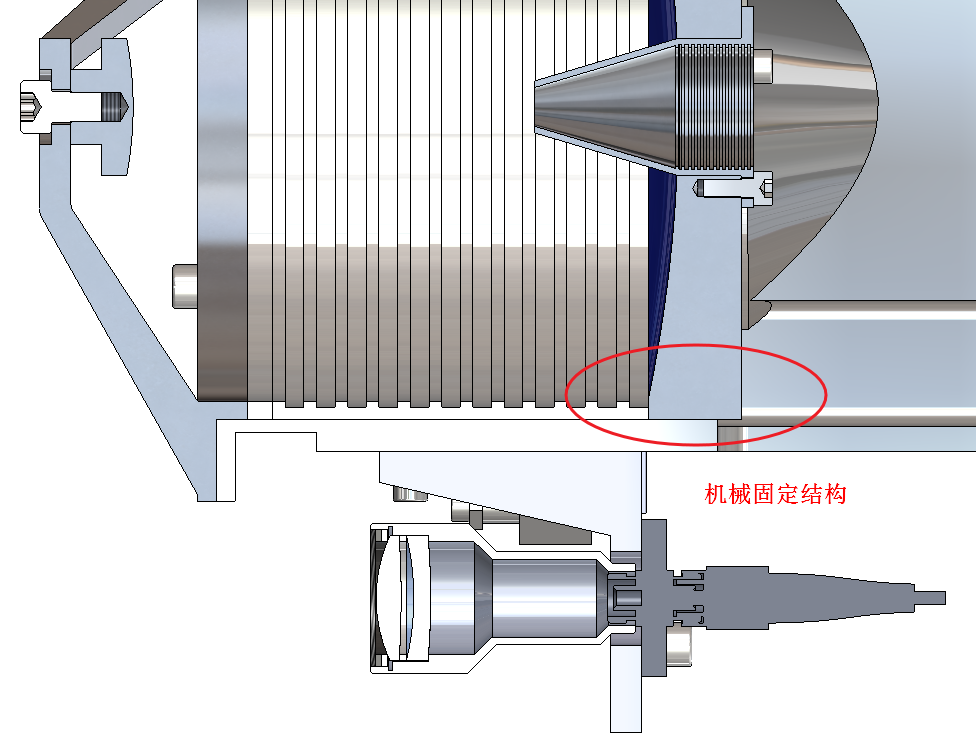
\includegraphics[width=\textwidth]{./Img/RCzhujing001.png}
		\caption{主镜光机结构剖面图}
		\label{RCzhujing001.png}
	\end{subfigure}%
	~%add desired spacing
	\begin{subfigure}[c]{0.5\textwidth}
		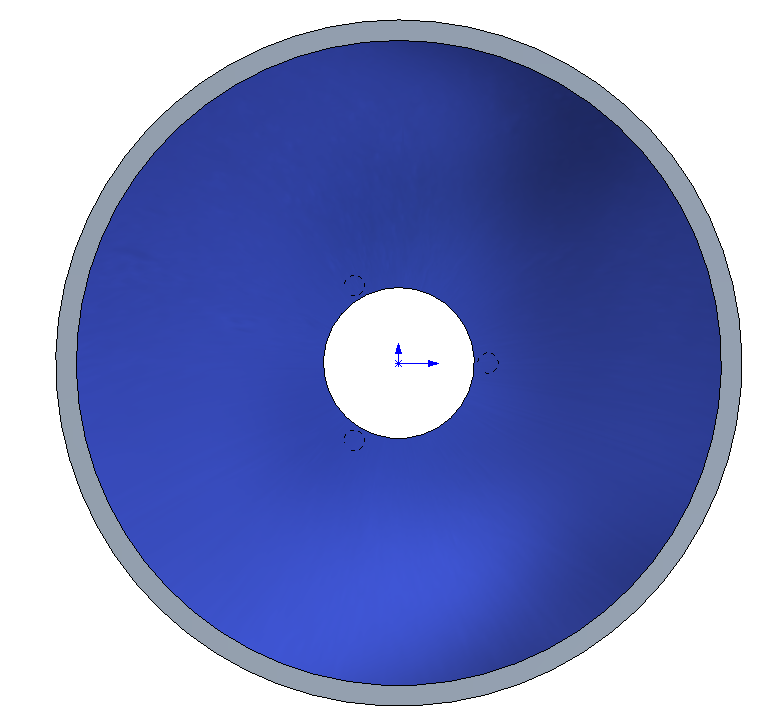
\includegraphics[width=\textwidth]{./Img/RCzhujing002.png}
		\caption{主镜光机结构图}
		\label{RCzhujing002.png}
	\end{subfigure}
	\caption{主镜光机结构}
%	\bicaption{主镜光机结构\ (a) 主镜光机结构剖面图,(b) 主镜光机结构图}{Primary Mirror Optical Machine Structure.(a) Cross-Section Drawn , (b) Machine Structure }
	\label{fig:MAIN-MIRROR}
\end{figure}

\subsection{次镜固定的机械结构设计}
RC望远系统次镜的设计主要在铁镍合金机械结构上镀高反射膜,并用弹性压圈把次镜压在次镜外筒上。如图所示\ref{RCcijing001.png}和\ref{RCcijing002.png}。
%\addimg{0.5}{RCcijing001.png}{次镜光机结构剖面图}
%\addimg{0.5}{RCcijing002.png}{次镜光机结构}
\begin{figure}[!htbp]
	\centering
	\begin{subfigure}[c]{0.5\textwidth}
		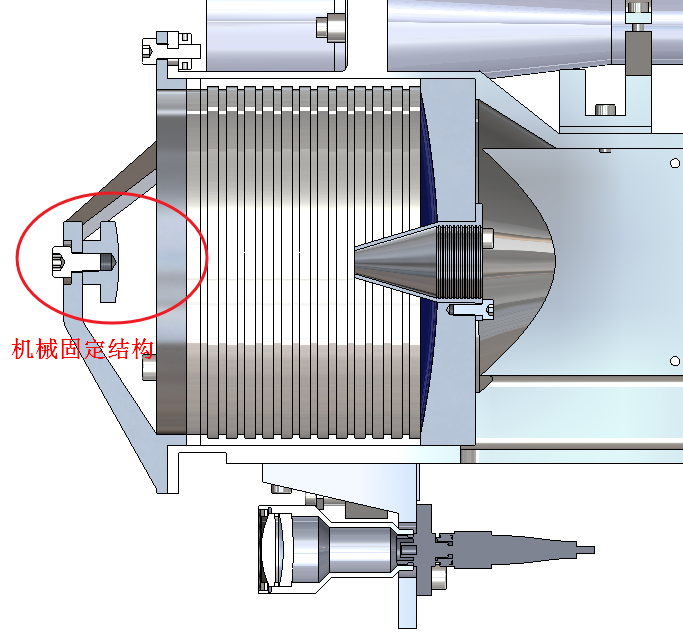
\includegraphics[width=\textwidth]{./Img/RCcijing001.png}
		\caption{次镜光机结构剖面图}
		\label{RCcijing001.png}
	\end{subfigure}%
	~%add desired spacing
	\begin{subfigure}[c]{0.5\textwidth}
		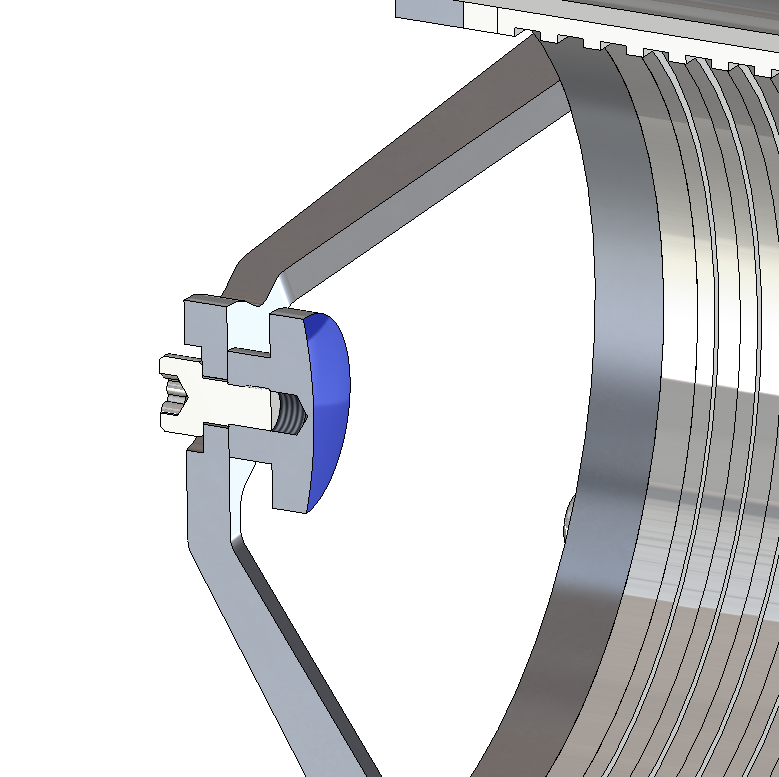
\includegraphics[width=\textwidth]{./Img/RCcijing002.png}
		\caption{次镜光机结构图}
		\label{RCcijing002.png}
	\end{subfigure}
	\caption{次镜光机结构}
%	\bicaption{次镜光机结构\ (a) 次镜光机结构剖面图,(b) 次镜光机结构图}{Primary Mirror Optical Machine Structure.(a) Cross-Section Drawn , (b) Machine Structure }
	\label{fig:Second-MIRROR}
\end{figure}

\section{装配误差}
载荷望远单元一定要考虑飞行器在地面操作、发射和飞行工作阶段的热环境和杋械环境下的公差。热离散和热梯度、材料变形、飞行器和光端机内部机械振动是引起光机装置轴线偏离的主要原因。在飞行工作阶段,热稳定性和机械稳定可以确保近衍射极限角工作状态。对准敏敏度的大部分信息可以通过光学设计软件获得。它包括了倾斜、间距、望远镜主镜和次镜的中心误差等。

在充分掌握热模型和结构模型后,辨别在不同环境条件下机械运动的角度,对光学对准偏差和波阵面误差预算就迎刃而解了。

为了使机载系统具有良好的稳定性,在光机装置在热设计和机械设计后,还要考虑位置公差要求,可以定量估计波前均方根误差(代表部分波长)。轴线偏差可以分为三类:单纯轴向偏差(如离焦);单纯横向偏差(如三级彗差);单纯倾斜偏差(也经常引入彗差)。在离焦时,光学主镜和次镜的轴线保持对准,仅是镜子间隔变化了。在横向偏差时,光学轴线不再重叠,而镜子间隔保持不变。后者的次镜轴线相对于主镜的轴线存在不同程度的倾斜和离心。

温度变化($\Delta T$)引起镜子材料的局部非弹性变化为$\alpha \Delta T$,其中α是热膨胀线性系数(CTE)。整个光机装置内部的平均温度变化使镜子的焦距(f)根据公式$\Delta f = f\alpha \Delta T$改变$\Delta f $。局部温度变化(梯度)导致局部表面变形,从而引发波前像差。

\section{光学系统的稳定性和轻小型化}
光机系统的微位移(几微米)会使成像质量达不到衍射极限。由于没有复杂系统的热模型,很难评价光学系统的热梯度影响。适当的热散可以减轻局部产生的热负载。由于整个光机系统可能经历很大的温度变化,如飞行器绕地球在轨运行(或另一个太阳系对象),太阳阴影和加热器常用于保持系统维持在恒定温度附近。望远镜口径越大,通过孔径的热梯度变化越明显,且很难在孔径内达到平衡。考虑空间使用要求(发射和接收),较大的光学孔径仅采取被动热稳定是不够的。

保持主一次镜的分离和重叠是避免受温度变化影响的一个关键设计因素。含有主动聚焦元件(尽管不可取)是一种降低光学轴线偏差的方法。同时,利用具有高导热系数的材料作为镜子的基底和结构也将减小热致轴线偏离。在这种情况下,太阳光照射在此结构上,反射光的热负荷会迅速传导出去。此外为了减少热效应,可选择热膨胀系数小的材料,如ULE、CER-VIT、CFRP、ZERODUR和SiC。例如,使用以碳化硅为基底材料的望远镜作为绝缘系统,它对热变化和梯度不敏感。热膨胀的残差造成离焦,可以采用适当热膨胀系数的材料(如一个特殊钢钢支架)来改变主一次镜子间的间隔从而进行补偿。

